\documentclass{a0poster}
\usepackage{fancytikzposter} 
 
\usepackage[T1]{fontenc} 
\usepackage[cp1251]{inputenc}
\usepackage[russian]{babel}
\usepackage{graphicx}
\usepackage{graphics}
\usepackage{amssymb}
\usepackage{mathtext}
\usepackage{caption}
\usepackage{subcaption}
\usepackage{setspace}
\usepackage{amsmath}
\usepackage{amsthm}
\usepackage{lscape}
\usepackage{makecell}
\usepackage{multirow}
\usepackage{ulem}
\usepackage{indentfirst}
\usepackage{enumerate}

\usepackage[margin=\margin cm, paperwidth=84.1cm, paperheight=118.9cm]{geometry}

%%%%% --------- Change here if you want ---------- %%%%%
%% margin for the geometry package, must be changed before using the geometry package
%% default value is 4cm
% \setmargin{4}

%% the space between the blocks
%% default value is 2cm
% \setblockspacing{2}

%% the height of the title stripe in block nodes, decrease it to save space
%% default value is 3cm
% \setblocktitleheight{3}

%% the number of columns in the poster, possible values 2,3
%% default value is 2
% \setcolumnnumber{3}

%% the space between two or more groups of authors from different institutions
%% used in \maketitle
% \setinstituteshift{10}

\usetemplate{3}

%% components of the templates
%% (the maximal possible numbers are mentioned as the parameters)
% \usecolortemplate{4}
% \usebackgroundtemplate{5}
% \usetitletemplate{2}
% \useblocknodetemplate{5}
% \useplainblocktemplate{4}
% \useinnerblocktemplate{2}


%% the height of the head drawing on top 
%% applicable to templates N3, 4 and 5
 \setheaddrawingheight{17}


%% change the basic colors
%\definecolor{myblue}{HTML}{008888} 
%\setfirstcolor{myblue}% default 116699
%\setsecondcolor{gray!80!}% default CCCCCC
%\setthirdcolor{red!80!black}% default 991111

%% change the more specific colors
\setbackgrounddarkcolor{colorone!70!black}
% \setbackgroundlightcolor{colorone!70!}
% \settitletextcolor{textcolor}
% \settitlefillcolor{white}
% \settitledrawcolor{colortwo}
% \setblocktextcolor{textcolor}
% \setblockfillcolor{white}
% \setblocktitletextcolor{colorone}
% \setblocktitlefillcolor{colortwo} %the color of the border
% \setplainblocktextcolor{textcolor}
\setplainblockfillcolor{colorone!10!}
% \setplainblocktitletextcolor{textcolor}
\setplainblocktitlefillcolor{colorone!60!}
% \setinnerblocktextcolor{textcolor}
% \setinnerblockfillcolor{white}
% \setinnerblocktitletextcolor{white}
% \setinnerblocktitlefillcolor{colorthree}

%% changing the fonts
%\usepackage{cmbright}

\renewcommand\normalsize{\fontsize{32}{39.8pt}\selectfont}

%% add your packages here
\usepackage{hyperref}

\title{ Bifurcations of zero balance state in one boundary-value problem \\
with deviation in edge condition }
\author{ \textit{ Leonid Ivanovsky \vspace{0.5cm}} \\
\textit{ P.G. Demidov Yaroslavl State University, \quad Scientific Center in Chernogolovka of RAS }
}

\begin{document}

%%%%% ---------- the background picture ---------- %%%%%
%% to change it modify the macro \BackgroundPicture
\ClearShipoutPicture
\AddToShipoutPicture{\BackgroundPicture}

\noindent % to have the picture right in the center
\begin{tikzpicture}
  \initializesizeandshifts
  % \setxshift{15}
  % \setyshift{2}

  %% the title block, #1 - shift, the default value is (0,0), #2 - width, #3 - scale
  %% the alias of the title block is `title', so we can refer to its boundaries later
  \ifthenelse{\equal{\template}{1}}{ 
    \titleblock{47}{1}
  }{
    \titleblock{47}{1.5}
  }

  %% a logo can be added to the title block
  %% #1 - anchor relative to the title block, #2 - shift, #3 - width, #3 - file name
  % \ifthenelse{\equal{\template}{2}}{ 
  %   \addlogo[south west]{(2,0)}{6cm}{unibz_b.png}
  % }{
  %   \addlogo[south west]{(2,0)}{6cm}{unibz_w.png}
  % }

  %%%%%%%%%% ------------------------------------------ %%%%%%%%%%
  \blocknodew{37}{ Boundary-value problem } %
  {
	\begin{equation}\label{ivanovsky-eq1}
		\dot{u} =  u'' + \gamma u - u^3,	
	\end{equation}
	\begin{gather}\label{ivanovsky-eq2}	
		u'(0, t) \, = 0, \\
		u'(1, t) \, = \alpha\,u(x_0, t), \nonumber
	\end{gather}
	$$ \alpha, \gamma \in \mathbb{R}, \quad x_0 \in [0, 1]. $$
	\vspace{0.4cm}	
  } 

  \blocknodew{37}{ Normal form } %
  {
	$$ \alpha = \alpha_{cr} + \varepsilon $$
	\begin{equation}\label{ivanovsky-eq3}
		u = \sqrt{\varepsilon}u_0 + \varepsilon u_1 + \varepsilon^{\frac{3}{2}} u_2 + O(\varepsilon^2)	
	\end{equation}
	
	$$ \sqrt{\varepsilon}: \; \dot{u_0} =  u_0'' + \gamma u_0 $$
	$$ u_0'(0, t) \, = 0 $$
	$$ u_0'(1, t) \, = \alpha_{cr}\,u_0(x_0, t) $$
  } 

  \blocknodew{37}{ Main result } %
  {	
    
    \vspace{1.9cm}  
    
	\begin{minipage}{\linewidth}
        \coloredbox{colorthree!150!}{\textbf{Theorem:} In the case of $ Re(\phi)>0,\, Re(d)<0 \;\; \exists \varepsilon_0 > 0 \;\; \forall \varepsilon \in (0,\varepsilon_0] $ there is observed an exponentially-orbitally stable cycle with asymptotic form $z(s) = \sqrt{-\frac{Re(\phi)}{Re(d)}} \exp{\left(i \left(Im(\phi) - \frac{Im(d)Re(\phi)}{Re(d)} \right) s + i\gamma \right)} $.}
     \end{minipage} 
     
     \vspace{1.5cm} 
     
  } 

	\blocknodew[($(currenty)+(19.5,0)$)]{76}{ Numerical results } %
  { 
  
  	\bigskip
	
	\hspace{-4cm}
	\begin{minipage}[h]{0.65\linewidth}
	\center{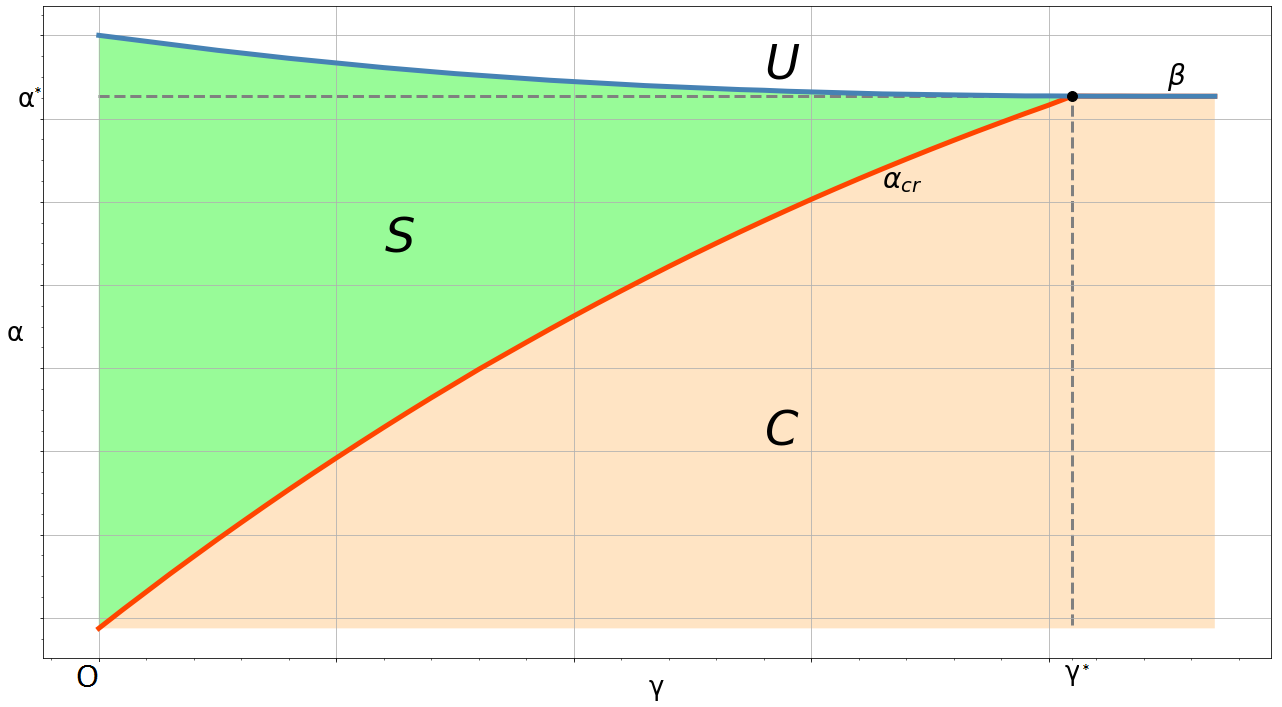
\includegraphics[width=0.65\linewidth]{scheme.png} }
	\end{minipage}	
	\hspace{-13cm}
	\begin{minipage}[h]{0.63\linewidth}
	\center{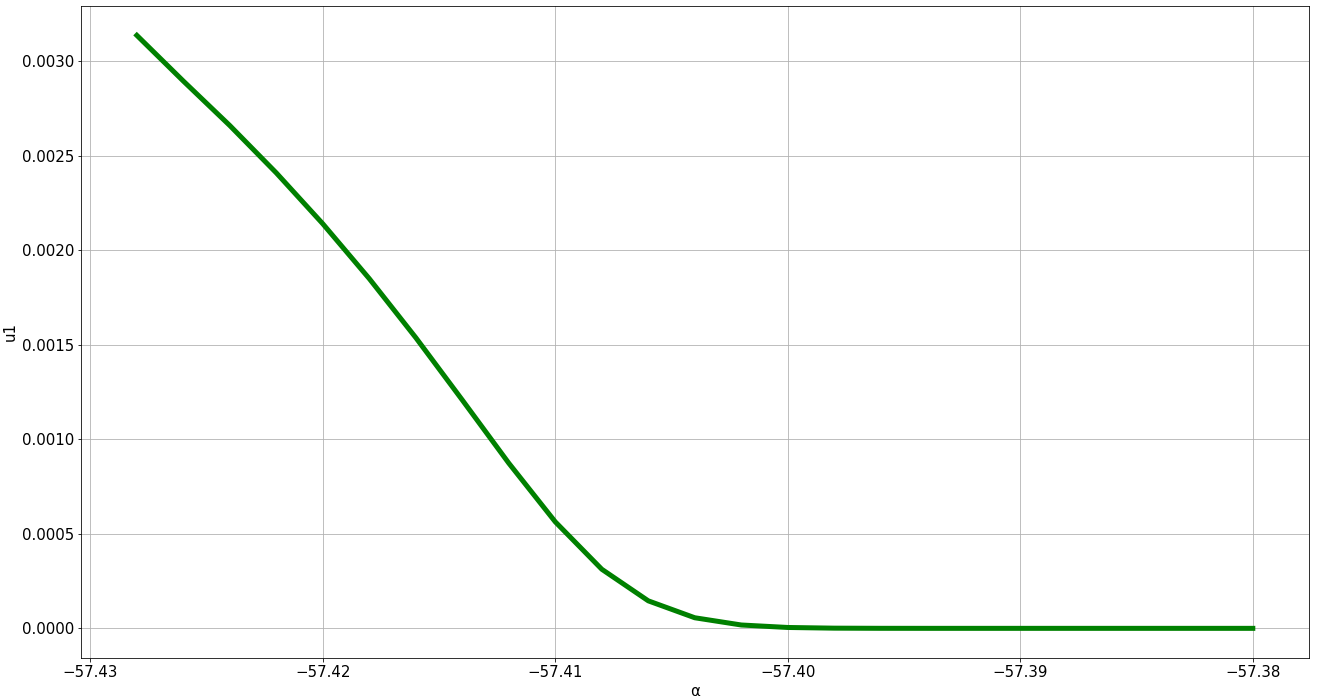
\includegraphics[width=0.63\linewidth]{points.png} \\ $ x_0 = 0{,}49, \; \gamma=2{,}4 $ }
	\end{minipage}
  
  }
  
  \blocknodew[($(currenty)$)]{76}{ Numerical results } %
  { 
	
	\hspace{-8cm}
	\begin{minipage}[h]{0.55\linewidth}
	\center{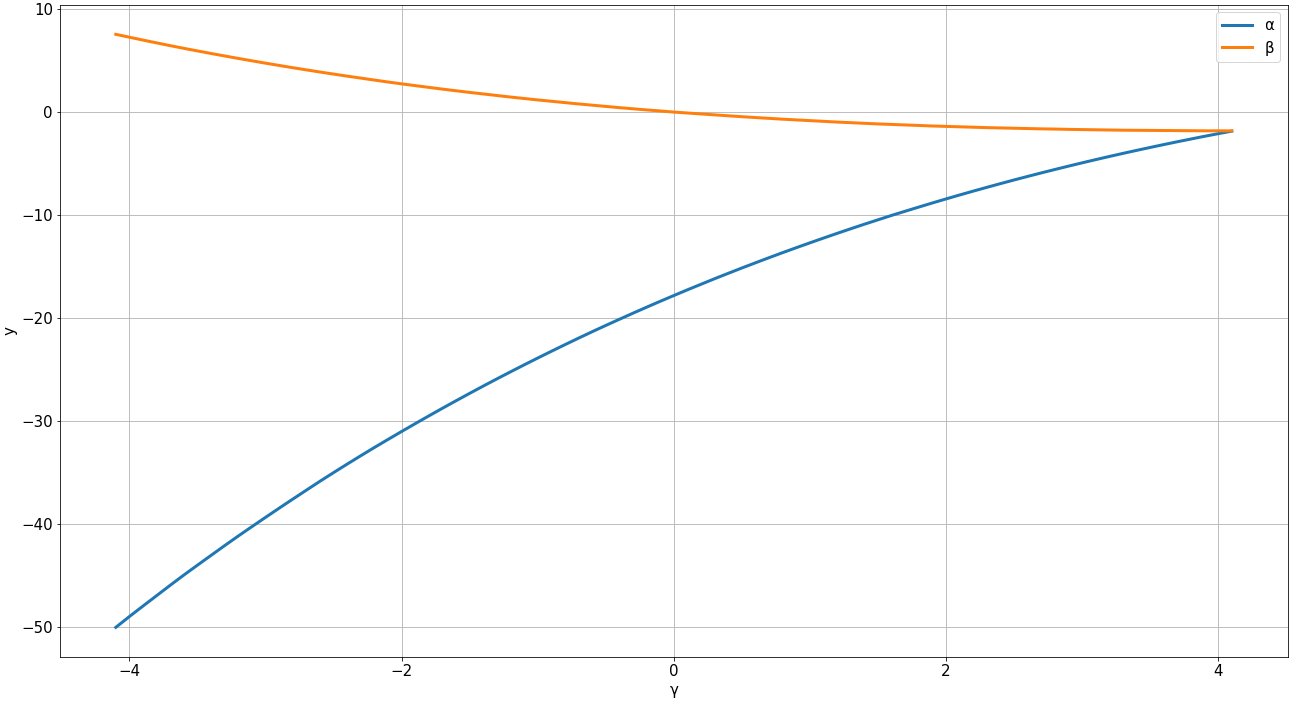
\includegraphics[width=0.55\linewidth]{x0=0,00.png} \\ a) $ x_0 = 0{,}0 $ }
	\end{minipage}	
	\hspace{-16.5cm}
	\begin{minipage}[h]{0.55\linewidth}
	\center{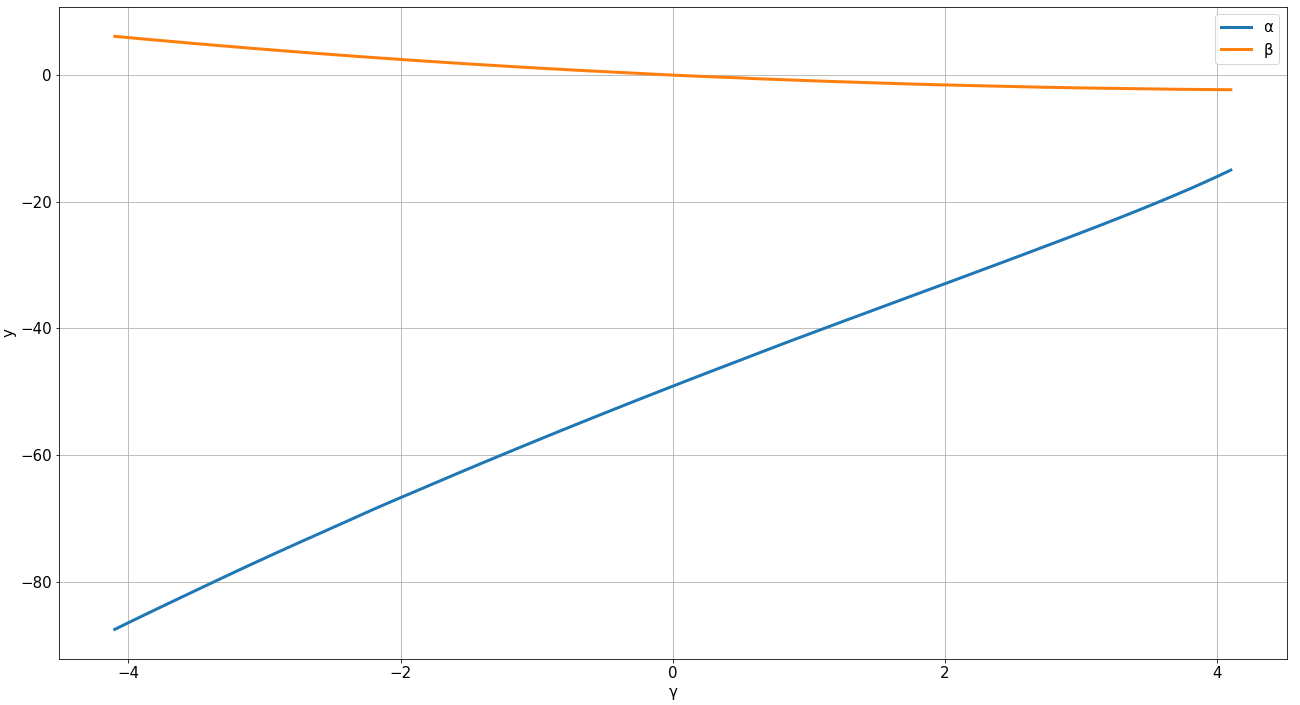
\includegraphics[width=0.55\linewidth]{x0=0,33.png} \\ b) $ x_0 = 0{,}33 $ }
	\end{minipage}
	\hspace{-16.5cm}
	\begin{minipage}[h]{0.55\linewidth}
	\center{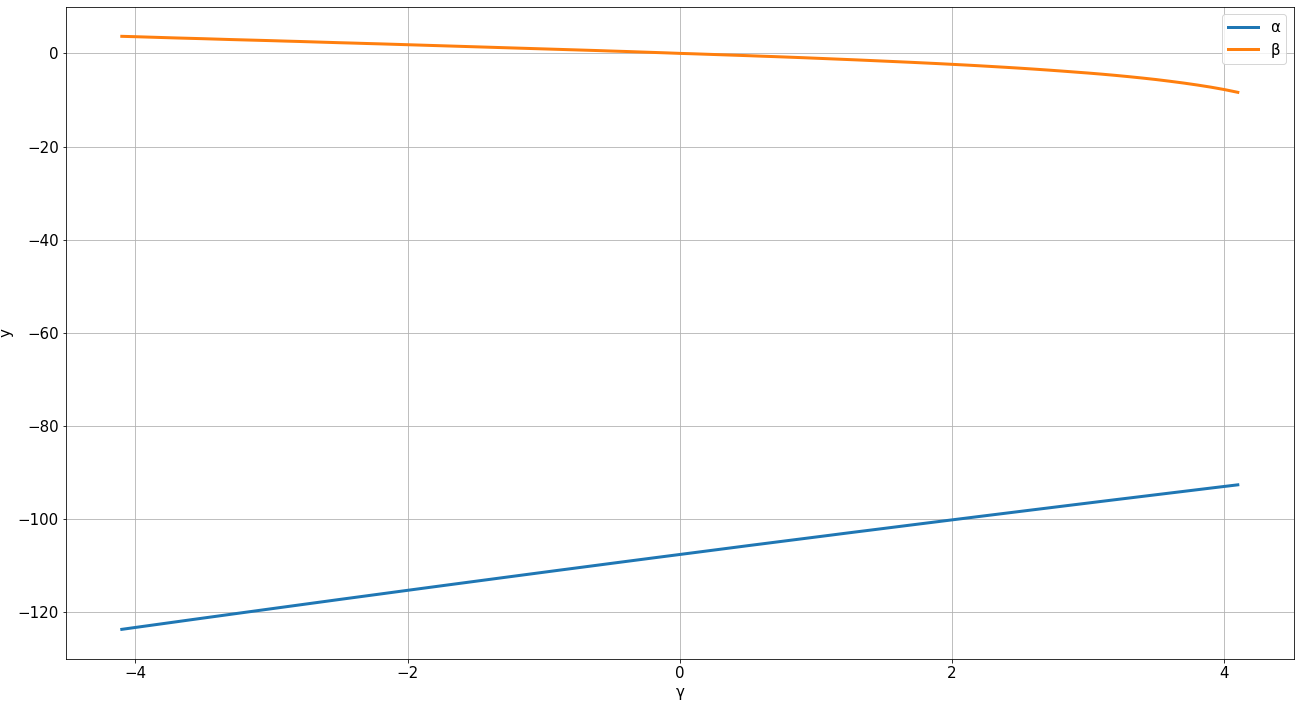
\includegraphics[width=0.55\linewidth]{x0=0,67.png} \\ c) $ x_0 = 0{,}67 $ }
	\end{minipage}
  
  }

  %%%%%%%%%%%%% NEW COLUMN %%%%%%%%%%%%%%% 
  \startsecondcolumn 

%%%%%%%%%% ------------------------------------------ %%%%%%%%%%
  \blocknodew{37}{ System for numerical experiments } %
  {
	
	\begin{equation}\label{ivanovsky-eq5}
		\dot{u}_j =  n^2(u_{j+1} - 2u_j + u_{j-1}) + \gamma u_j - u_j^3, \quad j = \overline{1, n},
	\end{equation}
	\begin{gather}\label{ivanovsky-eq6}	
		u_0 = u_1, \\
		u_{n+1} = 	u_n + \frac{\alpha}{n} u_k, \nonumber
	\end{gather}
	$$ k=k(x_0) \in \mathbb{N}, \quad k\in [1, n] $$
  }

  \blocknodew{37}{ Form for $u_0$ } %
  {
    \begin{equation}\label{ivanovsky-eq4}
		u_0 = z(s)e^{i\omega t}w(x) + \overline{z}(s)e^{-i\omega t}\overline{w}(x)
	\end{equation}  
	
   	$$ w(x) = c\,\mbox{ch}(\mu\, x), $$
   	 	
	$$ s = \varepsilon t, $$
	$$ \mu = \sqrt{\gamma+i\omega}, \quad \omega \in \mathbb{R}. $$
	\vspace{0.5cm}
  }

  \blocknodew{37}{ Form for $u_2$ } %
  {
	$$ \varepsilon^\frac{3}{2}: \quad z' e^{i\omega t} w + \dot{u}_2 = u''_2 + \gamma u_2 - (z e^{i\omega t}w + \overline{z} e^{-i\omega t}\overline{w})^3 $$
	$$ u_2'(0, t) \, = 0 $$
	$$ u_2'(1, t) \, = \alpha_{cr}\,u_2(x_0, t) + u_0(x_0, t) $$
	
	$$ z' = \phi z + d z |z|^2 $$
  } 

\end{tikzpicture}

\end{document}